\documentclass[12pt]{article}
\usepackage[top=1in, bottom=1in, left=.75in, right=.75in]{geometry}
\usepackage{amsmath, enumerate}
\usepackage{fancyhdr}
\usepackage{graphicx, xcolor, setspace}
\usepackage{txfonts}
\usepackage{multicol,coordsys,pgfplots}
\usepackage[scaled=0.86]{helvet}
\renewcommand{\emph}[1]{\textsf{\textbf{#1}}}
\usepackage{anyfontsize}
% \usepackage{times}
% \usepackage[lf]{MinionPro}
\usepackage{tikz,pgfplots}
\def\ra{\rightarrow}
\newcommand{\blank}[1]{\rule{#1}{0.75pt}}
\usetikzlibrary{calc,trees,positioning,arrows,fit,shapes,calc}
\pgfplotsset{width=9cm,compat=1.9}
\tikzset{
  jumpdot/.style={mark=*,solid},
  excl/.append style={jumpdot,fill=white},
  incl/.append style={jumpdot,fill=black},
}

\pgfplotsset{my style/.append style={axis x line=middle, axis y line=
middle, xlabel={$x$}, ylabel={$y$}}}

%axis equal

%yticklabels={,,} , xticklabels={,,}

% \setmainfont{Times}
% \def\sansfont{Lucida Grande Bold}
\parindent 0pt
\parskip 4pt
\pagestyle{fancy}
\fancyfoot[C]{\emph{\thepage}}
\fancyfoot[R]{v1} %%%%%% <-- Version Info
\fancyhead[L]{\ifnum \value{page} > 1\relax\emph{Math F251X: Midterm 2}\fi}
\fancyhead[R]{\ifnum \value{page} > 1\relax\emph{Spring 2025}\fi}
\headheight 15pt
\renewcommand{\headrulewidth}{0pt}
\renewcommand{\footrulewidth}{0pt}
\let\ds\displaystyle
\def\continued{{\emph {Continued....}}}
\def\continuing{{\emph {Problem \arabic{probcount} continued....}}\par\vskip 4pt}


\newcounter{probcount}
\newcounter{subprobcount}
\newcommand{\thesubproblem}{\emph{\alph{subprobcount}.}}
\def\problem#1{\setcounter{subprobcount}{0}%
\addtocounter{probcount}{1}{\emph{\arabic{probcount}.\hskip 1em(#1)}}\par}
\def\subproblem#1{\par\hangindent=1em\hangafter=0{%
\addtocounter{subprobcount}{1}\thesubproblem\emph{#1}\hskip 1em}}
\def\probskip{\vskip 10pt}
\def\medprobskip{\vskip 2in}
\def\subprobskip{\vskip 45pt}
\def\bigprobskip{\vskip 4in}


\newenvironment{subproblems}{%
\begin{enumerate}%
\setcounter{enumi}{\value{subprobcount}}%
\renewcommand{\theenumi}{\emph{\alph{enumi}}}}%
{\setcounter{subprobcount}{\value{enumi}}\end{enumerate}}


\newcommand{\be}{\begin{enumerate}}
\newcommand{\ee}{\end{enumerate}}


\begin{document}
{\emph{\fontsize{26}{28}\selectfont Spring 2025 \hfill
%{\fontsize{32}{36}\selectfont Calculus 1: Midterm 1}
\hfill Math F251X}}

\begin{center}
{\emph{%\fontsize{26}{28}\selectfont Spring 2024 
%%\hfill
{\fontsize{32}{36}\selectfont Calculus 1: Midterm 2}
%%\hfill Math F251X}
}}
\end{center}

%\vskip 2cm
\strut\vtop{\halign{\emph#\hskip 0.5em\hfil&#\hbox to 2in{\hrulefill}\cr
\emph{\fontsize{18}{22}\selectfont Name:}&\cr
%\noalign{\vskip 10pt}
%\emph{\fontsize{18}{22}\selectfont Student Id:}&\cr
%\noalign{\vskip 10pt}
%\emph{\fontsize{18}{22}\selectfont Calculator Model:}&\cr
}}
\hfill
\vtop{\halign{\emph{\fontsize{18}{22}\selectfont #}\hfil& \emph{\fontsize{18}{22}\selectfont\hskip 0.5ex $\square$ #}\hfil\cr
Section: & 9:15am (James Gossell)\cr
\noalign{\vskip 4pt}
         & 11:45am (Kevin Meek)\cr
\noalign{\vskip 4pt}
         & async (Deven Barnett)\cr}}

\vfill
{\fontsize{18}{22}\selectfont\emph{Rules:}}

\begin{itemize}
\item Partial credit will be awarded, but you must show your work.

\item You may have a single handwritten $3'' \times 5''$ notecard, both sides.

\item Calculators are {\bf not} allowed. 

\item Place a box around your  \fbox{FINAL ANSWER} to each question where appropriate.

\item Turn off anything that might go beep during the exam.

\end{itemize}

%If you need extra space, you can use the back sides of the pages.
%Please make it obvious  when you have done so.



Good luck!
\vfill
\def\emptybox{\hbox to 2em{\vrule height 16pt depth 8pt width 0pt\hfil}}
\def\tline{\noalign{\hrule}}
\centerline{\vbox{\offinterlineskip
{
\bf\sf\fontsize{18pt}{22pt}\selectfont
\hrule
\halign{
\vrule#&\strut\quad\hfil#\hfil\quad&\vrule#&\quad\hfil#\hfil\quad
&\vrule#&\quad\hfil#\hfil\quad&\vrule#\cr
height 3pt&\omit&&\omit&&\omit&\cr
&Problem&&Possible&&Score&\cr\tline
height 3pt&\omit&&\omit&&\omit&\cr
&1&&9&&\emptybox&\cr\tline
&2&&6&&\emptybox&\cr\tline
&3&&16&&\emptybox&\cr\tline
&4&&12&&\emptybox&\cr\tline
&5&&12&&\emptybox&\cr\tline
&6&&12&&\emptybox&\cr\tline
&7&&10&&\emptybox&\cr\tline
&8&&9&&\emptybox&\cr\tline
&9&&8&&\emptybox&\cr\tline
&10&&6&&\emptybox&\cr\tline \tline
&Extra Credit&&(5)&&\emptybox&\cr\tline
&Total&&100&&\emptybox&\cr
}\hrule}}}

\newpage

% Related Rates

\problem{9 points} The volume of a sphere is given by $\ds V=\frac{4}{3}\pi r^3 $ where $r$ is the radius of the sphere. If the radius is decreasing at a constant rate of 2 meters per second, find the rate at which the sphere's volume is decreasing when the radius is 5 meters. Include units in your final answer.

\begin{flushright}
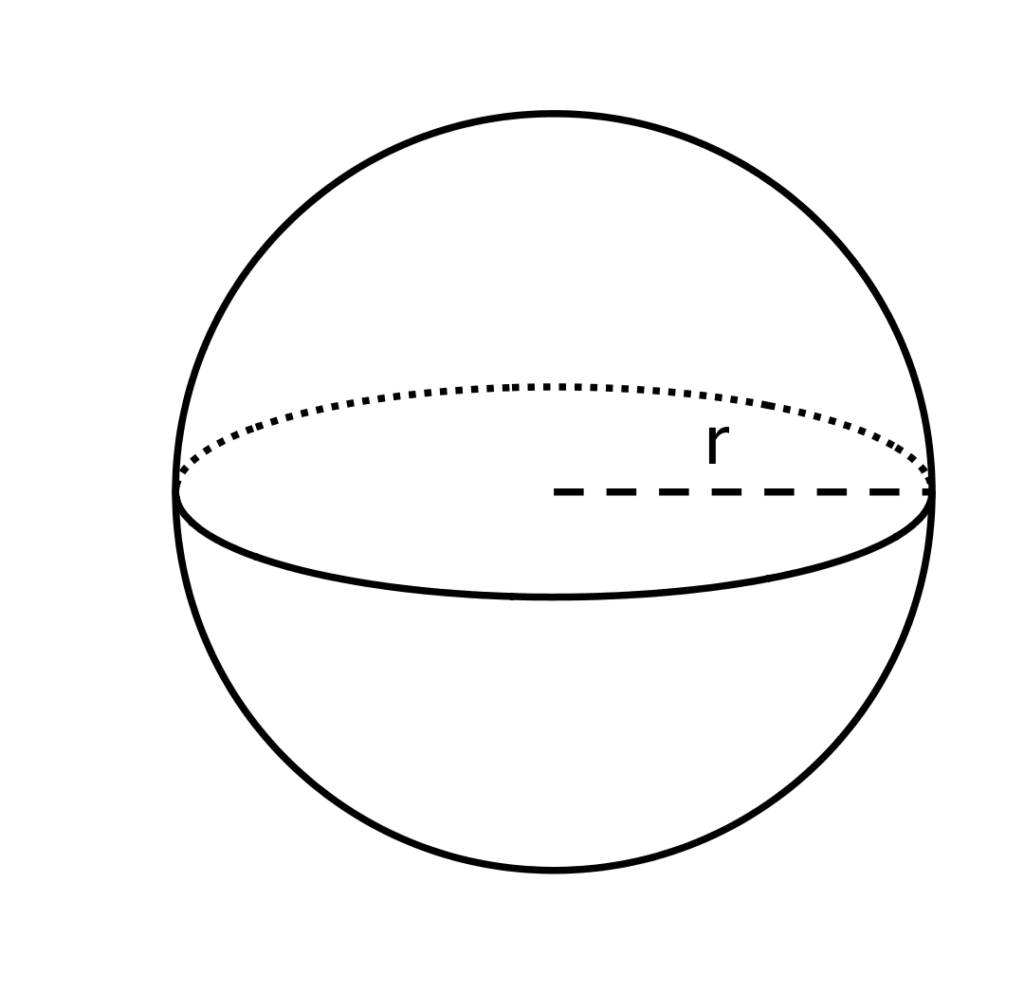
\includegraphics[width=0.3\textwidth]{Problem1Sphere.PNG} 
\end{flushright}

\vfill

% Max/Min Value

\problem{6 points} Let $g(x) = x + \cos(x)$. Determine the absolute maximum and absolute minimum of $g(x)$ on the interval $[0,2\pi]$. Justify your conclusion with work.
\vspace{1cm}

\vfill

  \begin{flushright}
    {\bf maximum value} of $g(x)$: \underline{\hspace{3cm}} \\
    \vspace{0.3cm}
    {\bf minimum value} of $g(x)$: \underline{\hspace{3cm}}
  \end{flushright}

\newpage


% Intervals of inc/dec/concavity, points

\problem{16 points} Let $\ds g(x) = x^{4/3} - 8x^{1/3}$. Note that we have
the following:
$$
g'(x) = \frac{4x-8}{3x^{2/3}} \qquad g''(x) = \frac{4x+16}{9x^{5/3}}
$$

{\bf You must show your work for all parts to receive credit!}
\begin{subproblems}
\item Determine the intervals where $g$ is {\bf increasing} and where
  $g$ is {\bf decreasing}.
  \vfill

\item Find the $x$ values where any {\bf local maxima} occur and where any
  {\bf local minima} occur.
  \vfill

\item Find the intervals where $g$ is {\bf concave up} and where $g$ is
  {\bf concave down}.
  \vfill

\item Find the $x$ values where any {\bf inflection points} occur.
  \vfill
\end{subproblems}

\newpage

% Limits

\problem{12 points}  Evaluate the following limits. \emph{Show your work}, including appropriate use of limit notation. If you use L'H\^opital's rule, you must indicate where you are using it by writing $\stackrel{H}{=}$ or $\stackrel{L'H}{=}$ or something similar. Use $\infty$ or $-\infty$ where appropriate, and if the limit does not exist, write {\sf DNE} and provide a justification.
\begin{subproblems}
	\item $\displaystyle \lim_{t \rightarrow \infty} \frac{ 2t^2-3t}{12-5t^2}$
	\vfill
	\item $\displaystyle \lim_{\theta \rightarrow 0} \frac{4\cos(\theta) - 4}{e^{\theta}-\theta-1}$
	\vfill
	\item $\displaystyle \lim_{x \rightarrow \infty} \frac{\sqrt{x}}{\ln (x^2 )} $
	\vfill
	\item $\displaystyle \lim_{x \rightarrow 0} x\cot x $
	\vfill
\end{subproblems}

\newpage

% Optimization

\problem{12 points} 

The surface area of a closed cylinder is given by $S = 2\pi r^2 +2\pi r h$ and the volume of a closed cylinder is given by $V = \pi r^2 h$ where $r$ is the radius and $h$ is the height of the cylinder. A packaging scientist is asked to design a cylindrical can with volume $36\pi$ cm$^3$ with the {\bf smallest possible surface area}.
\begin{subproblems}
	\item Write the expression to be minimized in terms of one variable.
	\begin{flushright}
	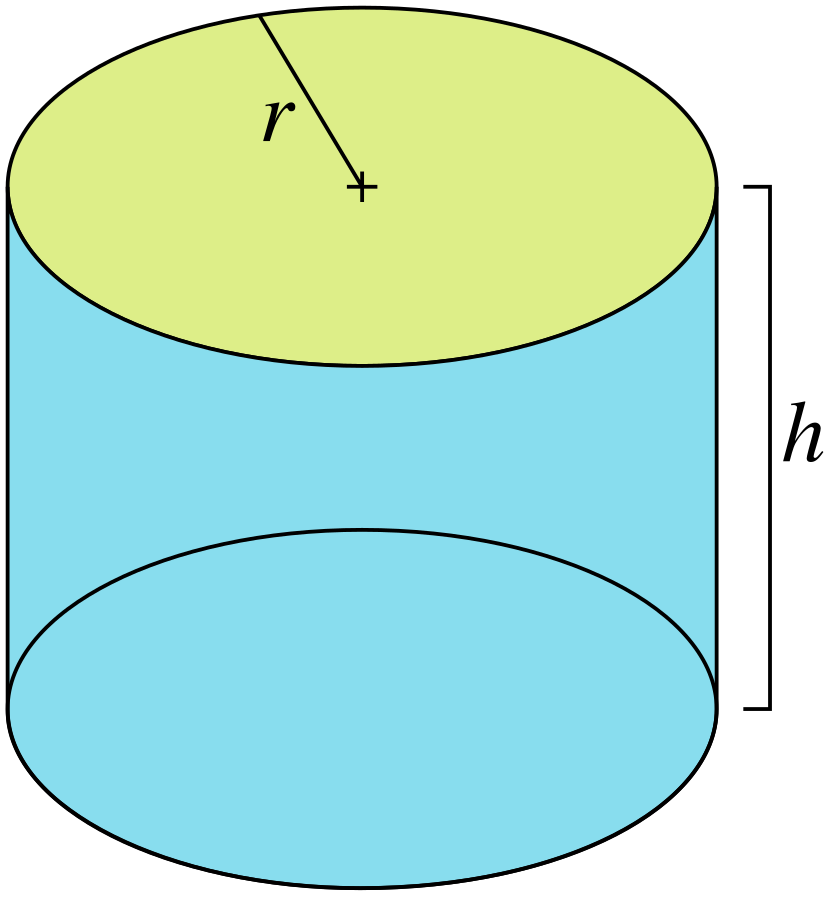
\includegraphics[width=0.2\textwidth]{Problem5Cylinder.PNG} 
	\end{flushright}
	\vspace{1cm}
	%\vfill
	\item Using calculus, find the radius and height of the cylinder with the smallest surface area. Justify that your answer gives the absolute minimum surface area.
	\vfill
	\vfill
	%\item Demonstrate that you have found the dimensions for the \textit{minimum} surface area.
	\vfill
	The dimensions of the cylinder with the minimum surface area are:\\
	
	\textbf{radius} = \blank{4cm} \hspace{1cm} \textbf{height} = \blank{4cm}
\end{subproblems}

\newpage

% Curve Sketching with properties

\problem{12 points} \emph{Sketch} a graph of a function $f(x)$ that satisfies all of the following properties.

After drawing the graph:
\begin{itemize}
\item \emph{Label} on the graph the following things, if they exist, by drawing a point on the graph and labeling: any local maximums by writing  \textsf{LOCAL MAX}, local minimums by writing \textsf{LOCAL MIN}, inflection points by writing \textsf{IP} 
\item Draw any horizontal and vertical asymptotes with dashed lines and \emph{label} them with their equation.
\item Mark any important $x$-values and $y$-values on the $x$- and $y$-axes.
\end{itemize}

\emph{Properties:}


\begin{multicols}{2}
\begin{itemize}
\item Domain is $(-\infty, 4) \cup (4, \infty)$
\item $f(1) =-1$, $f(-3) = 2$
\item $\ds{\lim_{x \to \infty} f(x) = 0}$
\item $\ds{\lim_{x \to -\infty} f(x) = 3}$
\columnbreak
%\item $f'(4)$ is undefined
\item $f'(x) > 0$ on $(0,4)$
\item $f'(x) < 0$ on $(-\infty,0) \cup (4, \infty)$
\item $f''(x) > 0$ on $(-2, 4) \cup (4,\infty)$
\item $f''(x) <0$ on $(-\infty,-2)$
\end{itemize}
\end{multicols}


\begin{tikzpicture}
\draw[<->] (-8,0) --  (8,0);
\draw[<->] (0,6) -- (0,-6);
\end{tikzpicture}

\newpage

  
% Integrals as Area

\problem{10 points} Consider the graph of the function $f(x)$ shown below:
	\vspace{-.5cm}
	\begin{center}
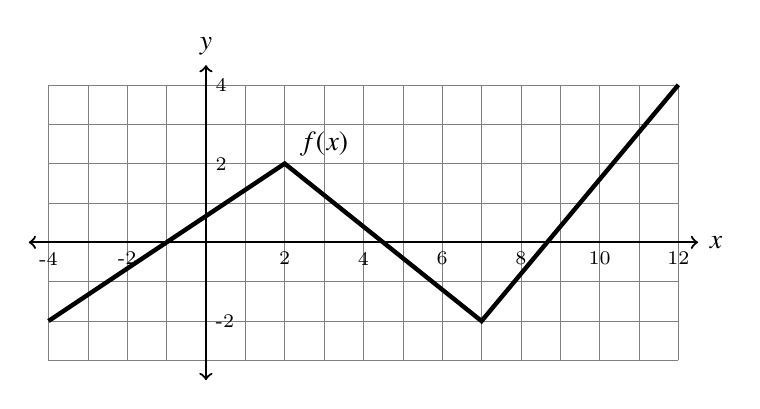
\begin{tikzpicture}[scale = .5]

\draw[help lines] (-4, -3) grid (12, 4);
\draw[thick,<->] (-4.5,0) -- (12.5,0) node[right] {$x$};
\draw[thick,<->] (0,-3.5) -- (0,4.5) node[above] {$y$};
%\draw[ultra thick] (5,0) -- (11,-3);
%\draw[ultra thick, -] (-4, 0) -- (-1,2) -- (7,-2) -- (12,3);
\draw[ultra thick, -] (-4, -2) -- (2,2) -- (7,-2) -- (12,4);
%\draw[ultra thick] (5,0) arc (0:180:5);
\foreach \i in { -4,-2,2,4,6,8,10, 12} {\path  (\i,0)node[below, font = \scriptsize] {\i};}
\foreach \i in {-2,2,4} {\path  (0, \i)node[right, font = \scriptsize] {\i};}
\node at (3,2.5) {$f(x)$};
\end{tikzpicture}
\end{center}

\begin{subproblems}
\item Determine $\ds{\int_{-1}^{7}f(x) \ dx}$. Show some work or say something about what you computed.

\vfill
\vfill

\item Determine $\ds{\int_{-1}^{7}(2f(x)+3)\ dx}$.  (Hint: Use part (a) above.)

\vfill
\vfill

\end{subproblems}

\newpage
  
% Indefinite integrals
  
\problem{9 points} Compute the following \emph{indefinite integrals} (antiderivatives). Give the most general answer, and show your work using correct notation.

\begin{subproblems}
	\item  $\displaystyle{ \int \sqrt[5]{x^{3}} + 3e^x - \cos(x)\: dx }$
	\vfill
	\item $\displaystyle \int x^2(3x+4) \: dx$
	\vfill
	\item $\displaystyle{ \int \frac{1-2x+4x^2}{x}\: dx  }$
	\vfill

\end{subproblems}

\newpage


% Applied Antiderivative

\problem{8 points} A drone is released into the air from an initial height of $5$ feet off the ground. Its upward velocity at $t$ seconds is given by $\displaystyle v(t) = \frac{1}{1+t^2}$ feet per second. $\left(\textit{Recall:   } \ds\frac{d}{dx}\arctan(x) = \frac{1}{1+x^2}\right)$.
\begin{subproblems}
\item How high will the drone be after $1$ second? Please include units in your answer.

\vfill

\item Compute $\displaystyle \lim_{t \rightarrow \infty} v(t)$, and write a sentence which interprets your result in the context of the problem.

\vfill

\end{subproblems}

\newpage

% Linear approximation

\problem{6 points}
Suppose we want to estimate $\sqrt{4.1}$.
\begin{subproblems}
  \item Find the linear approximation (linearization) of the
    function $f(x) = \sqrt{x}$ when $a=4$.
\vfill
  \item Use the linear approximation from part (a) to estimate
    $\sqrt{4.1}$. Your answer must be in the form of a simplified decimal
    or an exact fraction.
   \vfill
\end{subproblems}

% Extra Credit

\problem{Extra Credit: 5 points}
Compute $\displaystyle \lim_{x\to\infty} \sqrt{x^2-1}-x$. \emph{You must show your work}.

\vfill
\vfill
\vfill

\end{document}

%%%%ENDDOCUMENT


